\chapter{Nuevos ejercicios}
\label{chap:nuevos_ejercicios} 

\section{Sigue-líneas sofisticado}
Este ejercicio se basa en la propuesta realizada para la competición Robocup Junior Australia 2019\footnote{https://www.robocupjunior.org.au/}. Se trata de una versión mejorada del sigue-líneas usual en el que se incluyen trayectorias más complejas y diversas y dos niveles diferentes conectados a través de una rampa. \newline

Actualmente, este ejercicio está disponible en el entorno de \textit{Kibotics} para \textit{Python y Scratch} para el mBot. Además, gracias al motor de físicas complementario el robot es capaz de recrear un movimiento más realista durante la subida de la rampa. El controlador PD en velocidad del plano horizontal hace aplicar una fuerza más grande que la necesaria para avanzar en el suelo plano y, además, es necesario tener en cuenta el valor de la fricción para hacer más fácil o difícil la subida.

\begin{figure}[h!]
    \centering
    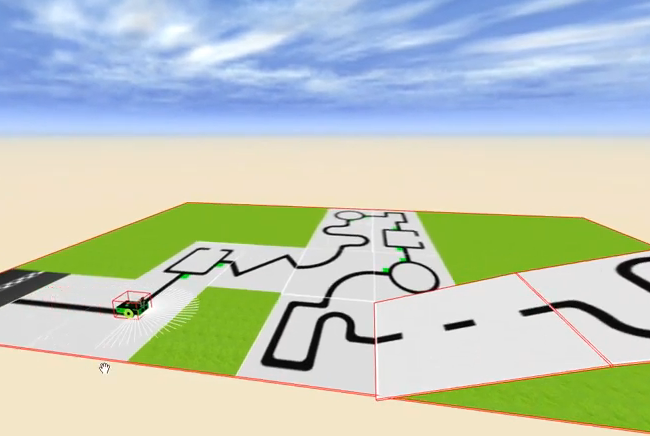
\includegraphics[width=0.6\textwidth, height=0.2\textwidth]{siguelineas.png}
    \caption{Sigue-líneas sofisticado}
    \label{fig:Sigue-líneas sofisticado}
\end{figure}

\section{ Laberinto 3D para mBot}
Este segundo ejercicio también se basa en la propuesta realizada para la competición Robocup Junior Australia 2019\footnote{https://www.robocupjunior.org.au/}.El objetivo de este ejercicio es hacer llegar al robot al punto en el que se encuentra otro robot perdido para rescatarle del laberinto. \newline

Este ejercicio está disponible en el entorno de \textit{Kibotics} para \textit{Python y Scratch} para el mBot. Además, se trata de un laberinto multinivel por lo que también se ve beneficiado por el motor de físicas complementario en la subida a través de la rampa.

\begin{figure}[h!]
    \centering
    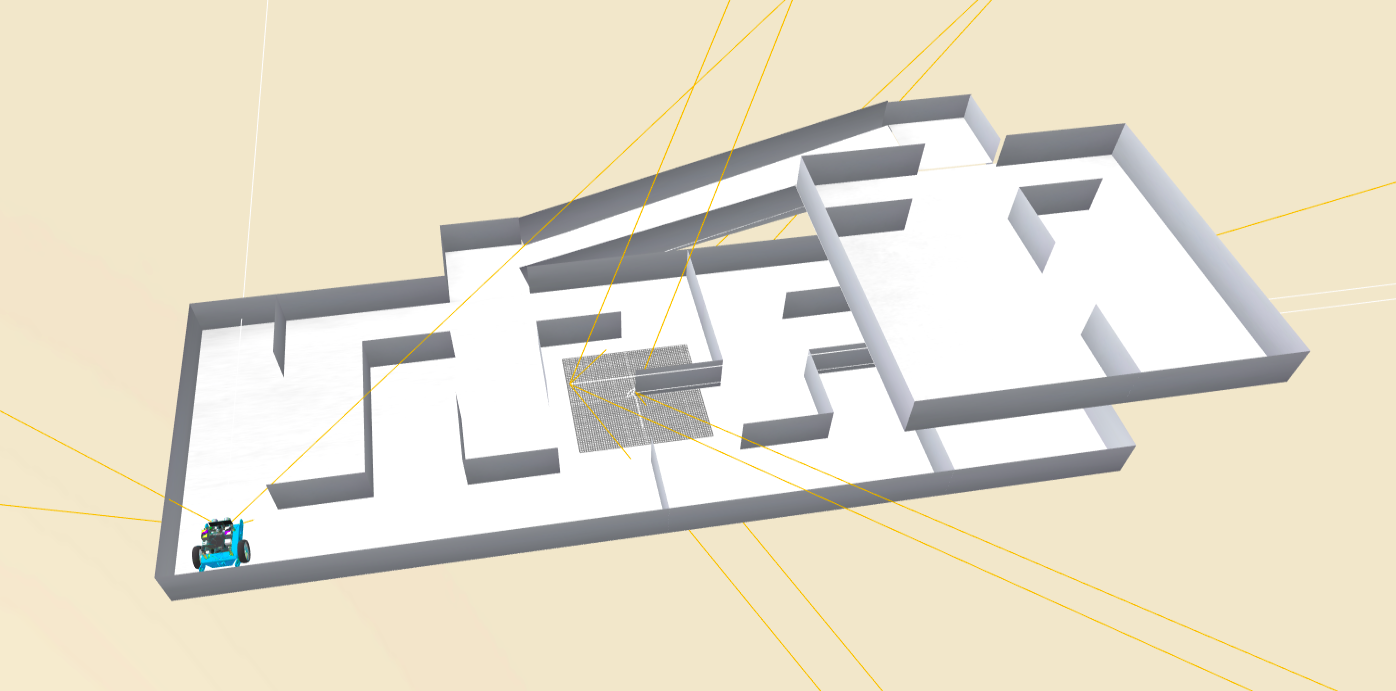
\includegraphics[width=\textwidth, height=0.8\textwidth]{laberinto.png}
    \caption{Laberinto 3D para mBot}
    \label{fig:Laberinto 3D para mBot}
\end{figure}


\section{Laberinto para drone}
Se han incluido dos ejercicios nuevos para el drone Tello. El objetivo de ambos ejercicios es que el drone encuentre la salida del laberinto. A continuación, se explican las dos versiones que se han realizado sobre este ejercicio.

\subsection{Sin señalización}
La primera versión está pensada para que el usuario logre hacer que el drone encuentre la salida mendiante el uso de instrucciones en posición. Por ejemplo, "avanza 2 metros", "gira a la derecha", etc.

\begin{figure}[h!]
    \centering
    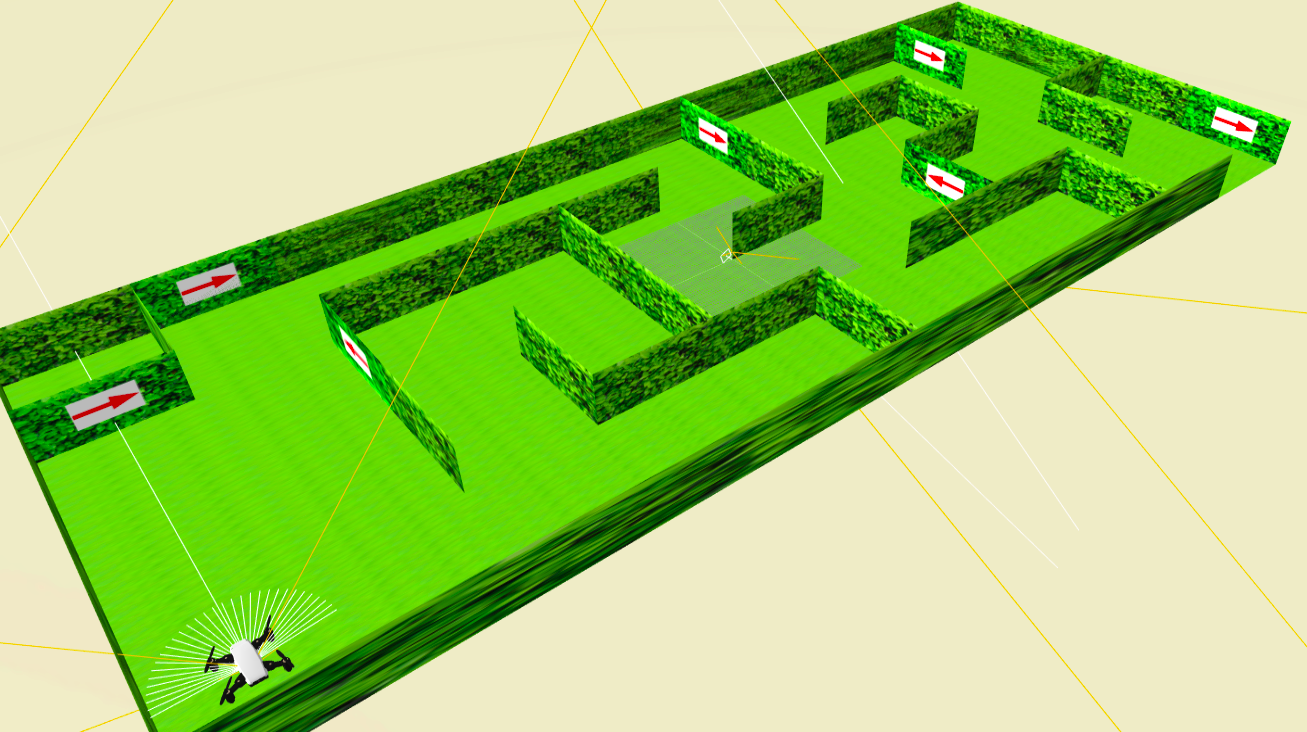
\includegraphics[width=\textwidth, height=0.8\textwidth]{laberinto_drone_flecha.png}
    \caption{Laberinto para drone con señalización}
    \label{fig:Laberinto_drone_señal}
\end{figure}

\subsection{Con señalización}
La segunda versión se ha implementado con el objetivo de que se utilicen los sensores y cámaras del drone para que se capten las señales que se han colocado por las paredes y que guían al drone para encontrar la salida. Gracias a la inteligencia artificial el drone será capaz de reconocer las señales y traducirlas en un movimiento determinado.

\begin{figure}[h!]
    \centering
    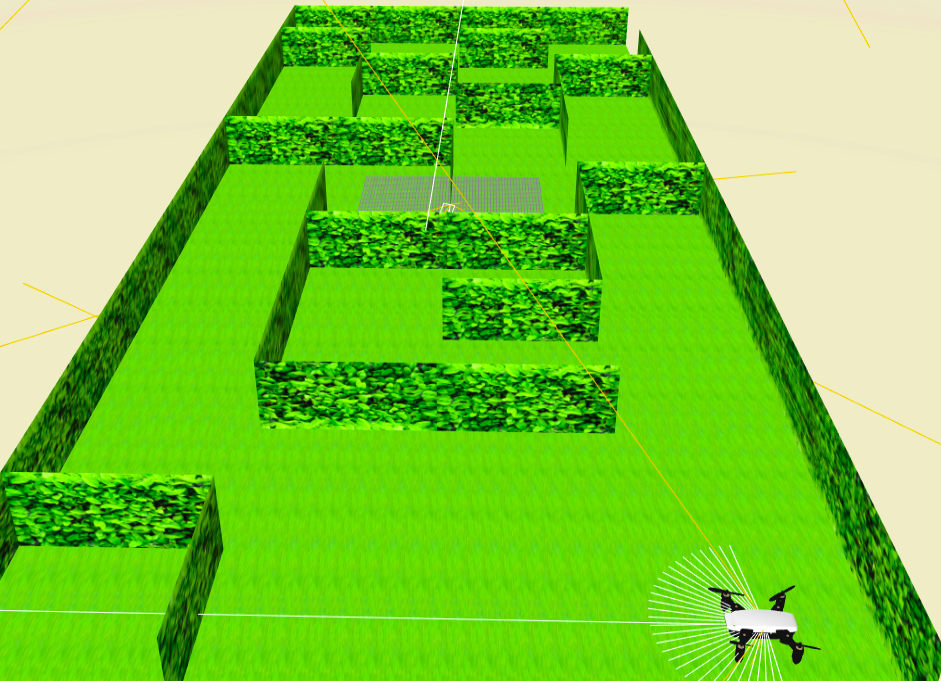
\includegraphics[width=\textwidth, height=0.8\textwidth]{laberinto_drone.png}
    \caption{Laberinto para drone sin señalización}
    \label{fig:Laberinto_drone}
\end{figure}

\section{Fútbol competitivo}
Este ejercicio también se basa en una de las propuestas presentadas para la competición Robocup Junior Australia 2019\footnote{https://www.robocupjunior.org.au/}. El objetivo de este ejercicio multijugador es meter más goles que el contrincante. El primero que llegue a diez goles será el ganador. Para ello, se ha implementado un evaluador que lleva la cuenta de los goles metidos por cada equipo\footnote{https://www.youtube.com/watch?v=lgwECFpTgNk}. 

\begin{figure}[h!]
    \centering
    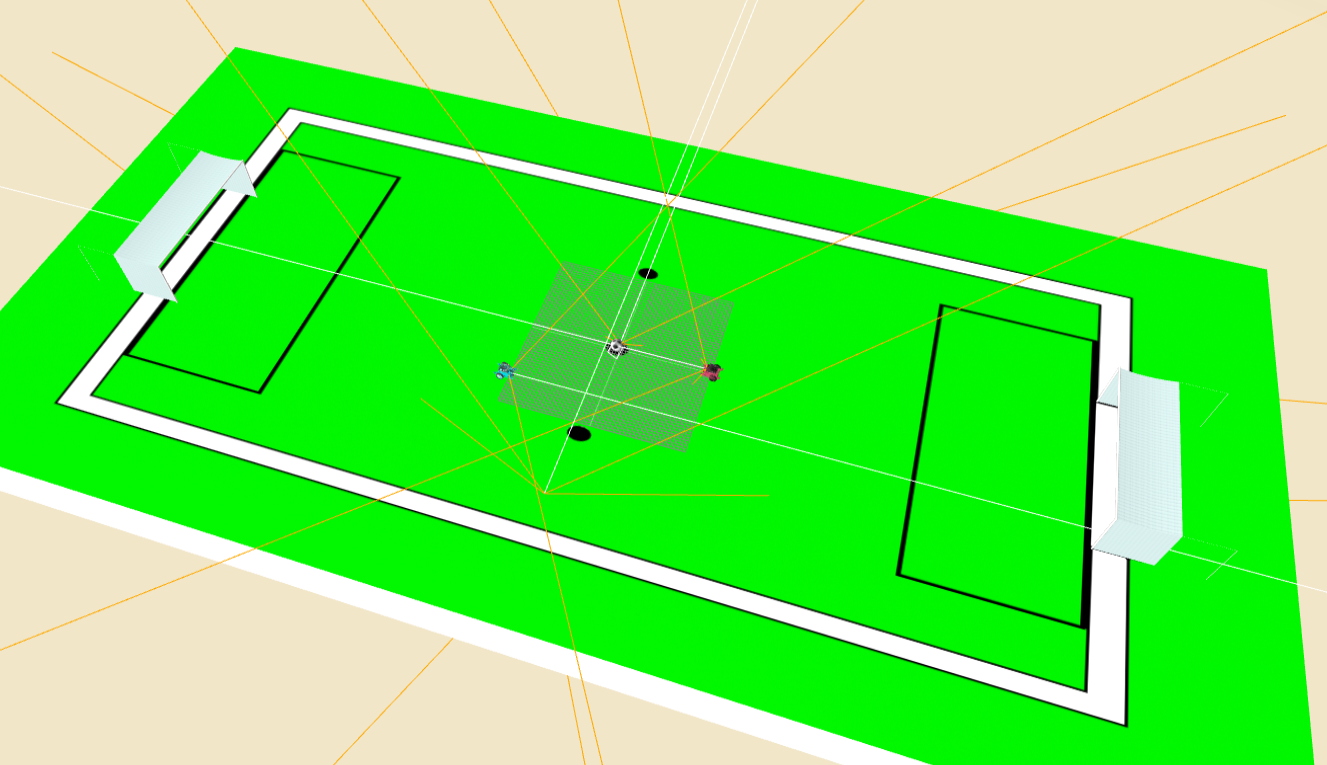
\includegraphics[width=0.8\textwidth, height=0.5\textwidth]{poteria.png}
    \caption{Fútbol competitivo}
    \label{fig:futbol}
\end{figure}

\begin{figure}[h!]
    \centering
    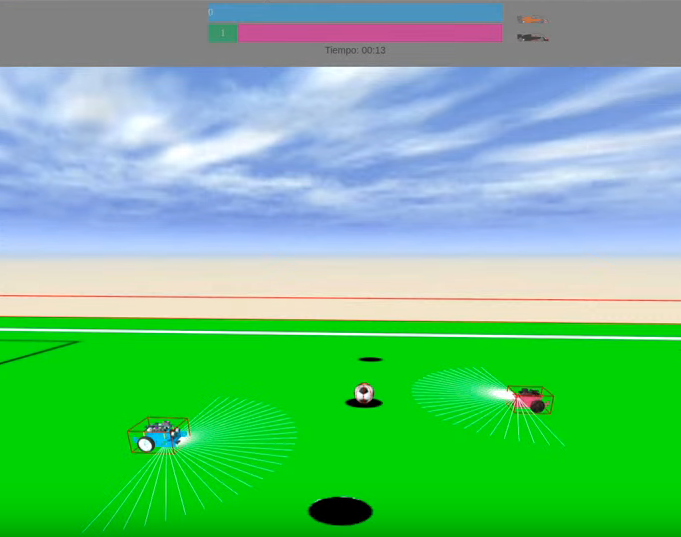
\includegraphics[width=0.8\textwidth, height=0.5\textwidth]{evaluador.png}
    \caption{Evaluador del ejercicio Fútbol competitivo}
    \label{fig:futbol}
\end{figure}

Este ejercicio saca provecho del estudio realizado en las físicas y del motor de físicas complementario tanto en los choques entre los robots y el balón como en el movimiento del balón. Ha sido necesaria la definición de un coeficiente de restitución adecuado para hacer realistas tanto los choques como el movimiento de la pelota. En este vídeo\footnote{https://www.youtube.com/watch?v=7W-FB3E0B_I} se observa un movimiento no realista del balón, mientras que en este otro\footnote{https://www.youtube.com/watch?v=PIJRqBGPeH4} se ha realizado el ajuste del coeficiente de restitución y la fricción, por lo que la pelota va girando sobre sí misma mientras va avanzando, haciendo mucho más realista el movimiento.

\section{Roomba}
Este ejercicio simula el funcionamiento de las aplicaciones hoy en día existentes para controlar la proporción de casa barrida por el robot Roomba. Para ello, se ha añadido un robot con el modelo de una aspiradora Roomba y un evaluador que calcula el porcentaje de habitación que ya ha sido barrida. El cómputo de dicho porcentaje se realiza mediante el empleo de un mapa de la habitación que almacena qué píxeles ya han sido barridos previamente\footnote{https://www.youtube.com/watch?v=ClxXPio05P4}.

\begin{figure}[h!]
    \centering
    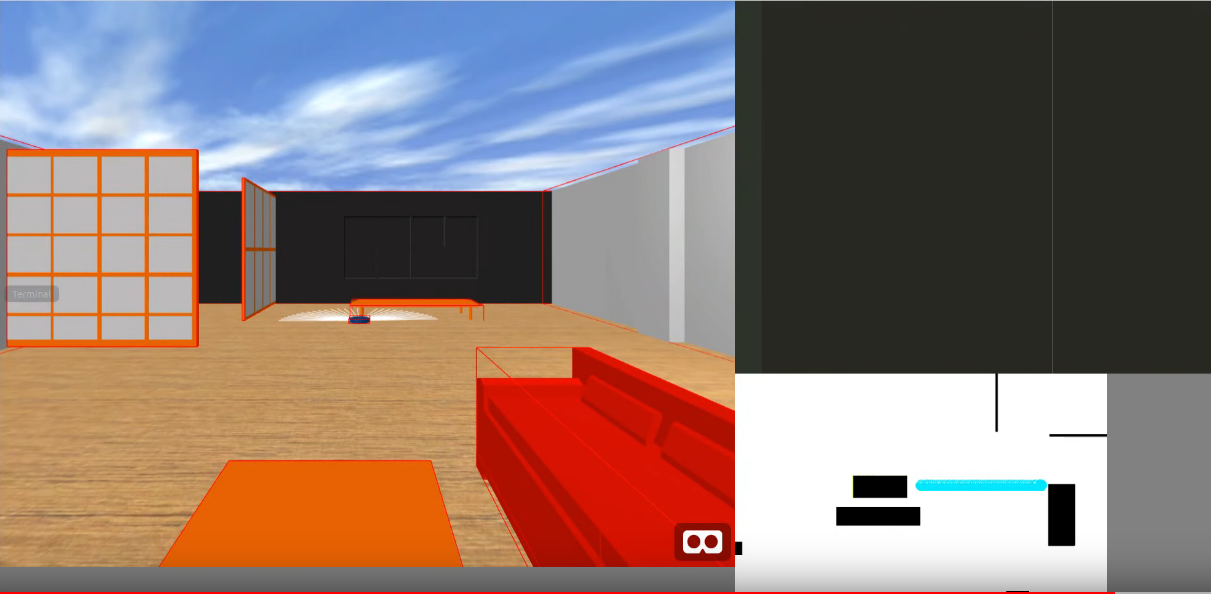
\includegraphics[width=0.9\textwidth, height=0.6\textwidth]{roomba_2.png}
    \caption{Roomba}
    \label{fig:roomba}
\end{figure}

\section{Aparcamiento}
El objetivo de este ejericio es que el piBot encuentre un sitio en este concurrido aparcamiento. Los modelos de los diferentes vehículos se han obtenido de las plataformas \textit{free3d}\footnote{www.free3d.com} y \textit{turbosquid}\footnote{www.turbosquid.com} y se han adaptado mediante la herramienta \textit{Blender}. El piBot deberá utilizar sus sensores de ultrasonidos para detectar si hay un coche aparcado en esa plaza o no. En el caso de que no haya ningún coche aparcado, el piBot efectuará la maniobra de aparcamiento.

\begin{figure}[h!]
  \begin{subfigure}[b]{0.4\textwidth}
    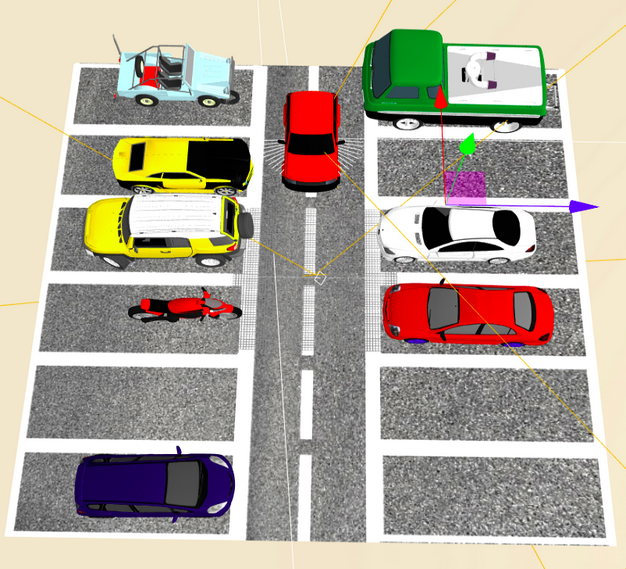
\includegraphics[width=\textwidth, height=\textwidth]{park.png}
    \caption{Ejemplo de coches aparcados}
  \end{subfigure}
    \hfill
  \begin{subfigure}[b]{0.4\textwidth}
    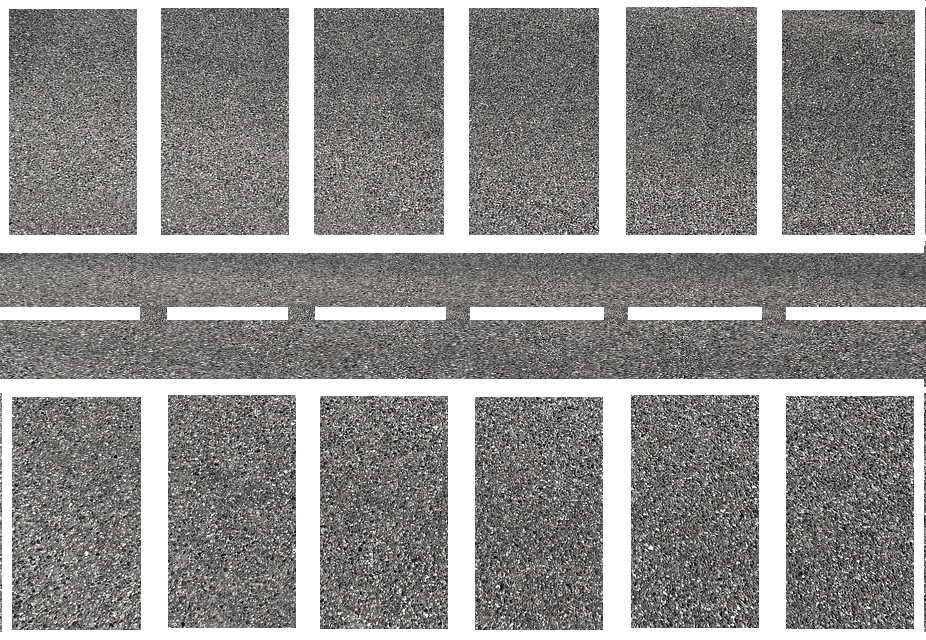
\includegraphics[width=\textwidth, height=\textwidth]{suelo_aparcamiento.jpg}
    \caption{Suelo del aparcamiento}
  \end{subfigure}
    \hfill
\caption{Aparcamiento}
\label{fig:aparcamiento}
\end{figure}



